\chapter{Korištenje funkcija u Tex-u}

Sadržaji koji se mogu uključiti u Priloge su: izvođenje jednačina i formula, detalji važnijih softverskih programa, razne tabele i dijagrami, karkateristike i performanse ili opisi opreme i komponenti koje su korištene u disertaciji/radu. Mogu se takodjer uključiti konstrukcioni crteži ili električne sheme.

U ovom prilogu prikazane su neke od funkcije koje se mogu koristiti prilikom oblikovanja rada i prikaza rezultata istraživanja korištenjem \LaTeX a. 


\section{Matematički izraz}


Primjer matematičke formule prikazan je izrazom

\begin{equation}
  T: \mathbf{x}_B \mapsto \mathbf{x}_A \Leftrightarrow T(\mathbf{x}_B) = \mathbf{x}_A.
  \label{eq:transformacija}
\end{equation}

Matematičke relacije se u \LaTeX razvojnom okruženju automatski numeriraju. Međutim, da bi se pojedina relacija (slika, tabela) referencirala u tekstu, potrebno je da se svakoj relaciji (slici, tabeli) dodijeli pogodna labela npr. {\tt {\textbackslash label\{MojaRelacija\}}}, a potom referencira u .tex fajlu sa {\tt {\textbackslash ref\{MojaRelacija\}}}. Na taj način će se \LaTeX pobrinuti za odgovarajuće kros-referenciranje.

\section{Slika}
Slika \ref{fig:Slika_citat} služi kao primjer uključivanja slike \index{uključivanje slike} u tekst. Relacije, slike i tabele se automatski numeriraju u \LaTeX u, i to sa oznakom brojpoglavlja.brojslike (npr. u Poglavlju 3 se numeriraju sa 3.1, 3.2, ... neovisno od toga u kojoj sekciji ili podsekciji se nalaze).

\begin{figure}
  \centering
  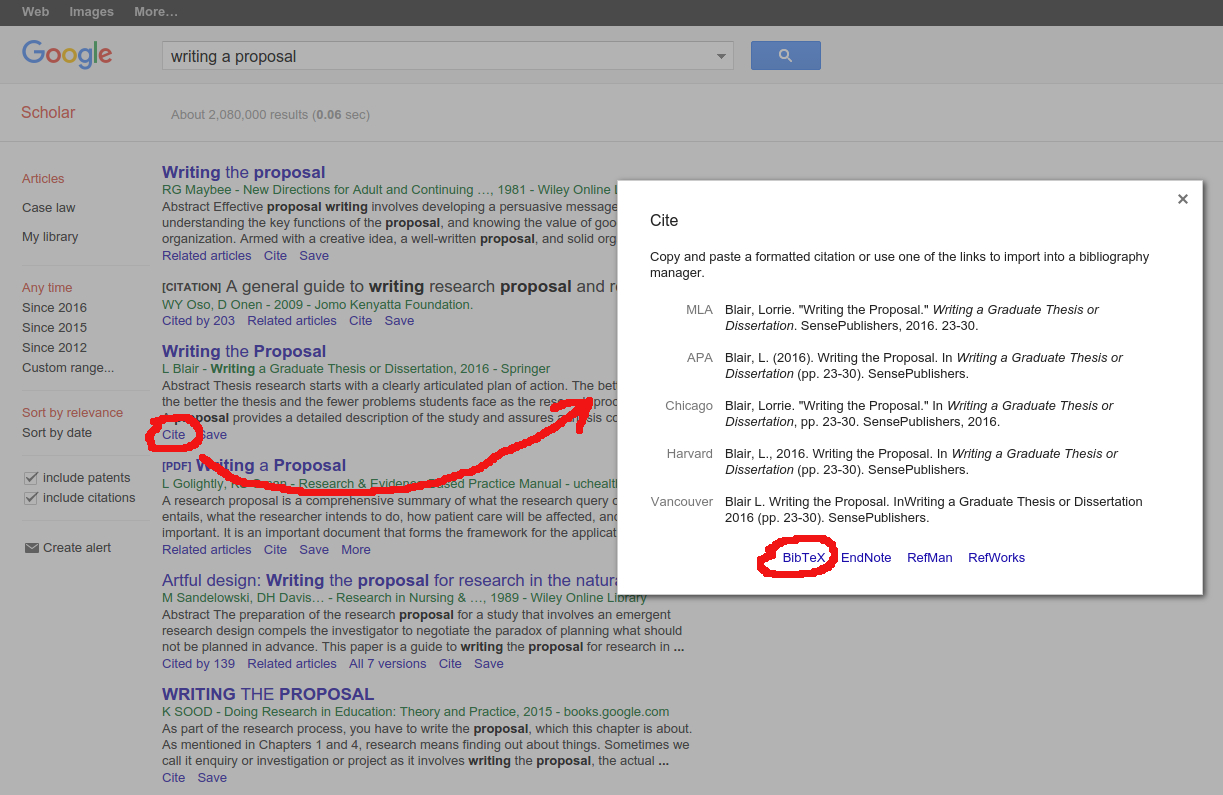
\includegraphics[width=0.7\textwidth]{SlikaCitat}
  \caption{Primjer naslova slike - uputstvo za traženje bibiografskih referenci na Google Scholar.}
  \label{fig:Slika_citat}
\end{figure}

\begin{figure}
  \centering
  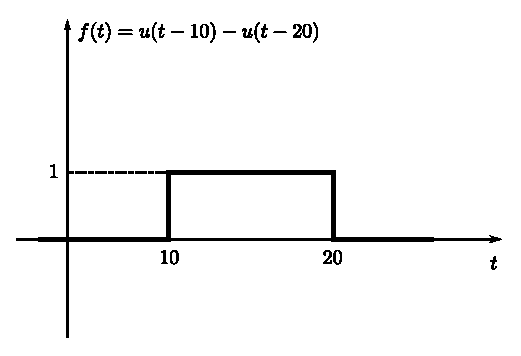
\includegraphics[width=0.5\textwidth]{SlikaCitat3}
  \caption{Primjer dijagrama - veličina i tip fonta na slici bi trebao odgovarati veličini i tipu fonta u tekstu}
  \label{fig:Slika_citat_3}
\end{figure}


\section{Tabela}
Formiranje tabele prikazano je na primjeru u Tabeli \ref{tab:confusion_matrix}. Za razliku od naslova slika, naslov tabela stoji iznad odgovarajućih tabela u tekstu.
\renewcommand{\arraystretch}{1.5} % prosirivanje redova u tabeli
\begin{table} [!ht]
  \caption{Naslov tabele}
  \begin{center}
  \begin{tabular}{ | c | c | c | c |}
	\hline
    Oznaka reda & Kolona 1 & Kolona 2 & Kolona 3 \\
    \hline 
    \hline
    red 1 & 1 & 2 & 3 \\ 
    \hline
    red 2 & 3 & 2 & 1 \\ 
     \hline
    red 3 & $E=mc^2$ & 2 & 3 \\ 
     \hline
  \end{tabular}
  \label{tab:confusion_matrix}    
\end{center} 
\end{table}
\renewcommand{\arraystretch}{1} % vraćeno na staro

\section{\textit{Landscape}}

Postavljanja stranice u prikaz \textit{landscape} prikazano je umetanjem izduzene Slike \ref{fig:Slika_citat2} u \textit{landscape} format papira. 

\begin{landscape}
 \begin{figure}
  \centering
  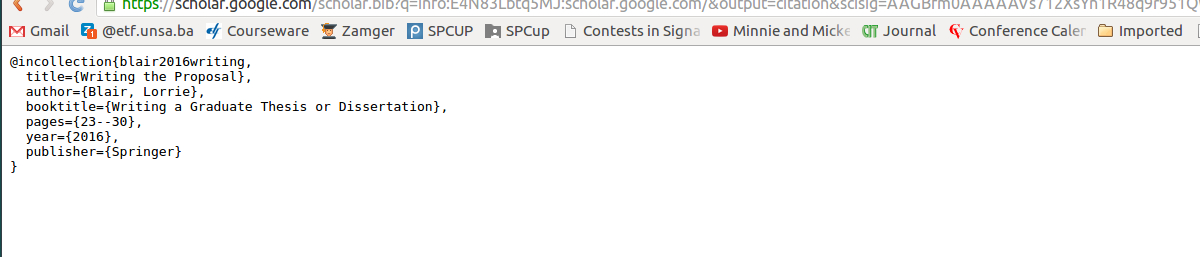
\includegraphics[width=25cm]{SlikaCitat2}
  \caption{Primjer ekstrakcije bibliografskih stavki za kopiranje u .bib fajl, sa Google Scholara}
  \label{fig:Slika_citat2}
\end{figure}
\end{landscape}

\section{Indeks pojmova i Popis oznaka}

Ukoliko je u radu neophodno uvesti i indeks, odnosno popis oznaka, onda se to radi na sljedeći način. Prilikom definiranja indeksa koristi se {\tt \textbackslash index\{ime\}}. Npr. {\tt \textbackslash index\{uključivanja slike\}}. 

Kod dodavanja pojmova u Popis oznaka u .tex fajlu se koristi {\tt \textbackslash nomenclature\{simbol\} \{opis\}}, npr. {\tt \textbackslash nomenclature\{ETF\}\{Elektrotehnički fakultet\}}.
Generiranje indeksa i Popisa oznaka se pravi korištenjem naredbi {\tt \textbackslash makeindex} i {\tt \textbackslash makenomenclature} u preambli, odnosno {\tt \textbackslash printindex} i {\tt \textbackslash printnomenclature} na mjestu generiranja popisa. 
Osim toga, potrebno je i kompajlirati dokument sa MakeIndex. 




\section{Korištenje literature}

Popis literature navodi se na kraju rada. Da bi uz \LaTeX  efikasno koristila literatura, potrebno je da se generira fajl sa bibliografskim jedinicama. Fajl {\tt literatura.bib} je sastavni dio ovog rada, i može poslužiti kao primjer kako se pišu pojedine bibliografske jedinice. Svaki unos (referenca) sadrži labelu na tu referencu, putem koje se bilo gdje u radu može citirati npr. sa {\tt \textbackslash cite\{Hajn01\} }. 

Dobar trik za popunjavanje bibliografskih unosa u .bib fajlu je korištenje Google Scholara \url{https://scholar.google.com/}. Osim što je baza naučnih radova, Google Scholar omogućava i kopiranje zapisa referenci na ispravan način. Podržani su svi najpopularniji formati citiranja (MLA, Chicago, Harvard itd.), kao što se vidi na Slici \ref{fig:Slika_citat}. Osim toga, klikom na dugme "BibTeX", moguće je izabrati i zapis reference razumljive razvojnom okruženju \LaTeX, a nakon toga je jednostavno kopirati u bibliografski fajl  {\tt literatura.bib} (vidjeti Sliku \ref{fig:Slika_citat2}).

Primjeri navođenja literature su knjiga \cite{Hajn01}, poglavlje u knjizi \cite{Samp05}, članak objavljen u časopisu \cite{Sim03}, članak objavljen na konferenciji \cite{Wirt99}, doktorski rad \cite{Will93}, Internetski izvor \cite{Jone12} te različite druge publikacije \cite{Rsoft}. Stil navođenja literature temelji se na stilu razvijenom za IEEE časopise i konferencije.

\section{Programski kodovi}

Programski kodovi se \LaTeX u navode korištenjem okruženja {\tt lstlisting}. Primjer koda je dat ispod.

\begin{lstlisting}[frame=single,language=C++,numbers=left, numberstyle=\tiny, xleftmargin=0.05\textwidth, xrightmargin=0.05\textwidth, basicstyle=\ttfamily\footnotesize, caption=Primjer programa]
// program u C++
#include <iostream>

int main ()
{
  std::cout << "Dobar Dan! ";
  std::cout << "Prvi program u C++";
}
\end{lstlisting}
